\documentclass[11pt]{article}

% Layout
\usepackage[margin=1in]{geometry}
\usepackage{setspace}
\onehalfspacing

% Packages
\usepackage{lmodern}
\usepackage{amsmath,amssymb}
\usepackage{booktabs}
\usepackage{graphicx}
\usepackage{hyperref}
\usepackage{xcolor}
\usepackage{natbib}
\usepackage{multirow}
\usepackage{enumitem}
\usepackage{caption}
\usepackage{subcaption}

\hypersetup{colorlinks=true, linkcolor=blue!60!black, citecolor=green!50!black, urlcolor=blue!70!black}

\title{\textbf{The Other Half of Intelligence:} \\
\large System Architecture as an Orthogonal Axis of AI Capability}

\author{
  Helo Ren \\
  Hestia's Creations \\
  \texttt{helo@hestiascreations.com}
}

\date{February 2026 — Working Draft}

\begin{document}
\maketitle
\thispagestyle{empty}

% ============================================================================
\begin{abstract}
The dominant paradigm in AI capability research focuses on scaling: larger models, longer context windows, better reasoning chains. We demonstrate that this captures only half the picture. Through systematic experiments on multi-hop question answering, we show that \emph{system-level decomposition}---where a complex question is broken into single-hop sub-questions handled by separate retrieval-extraction cycles---produces dramatic improvements across models spanning three orders of magnitude. A 7B parameter model improves from 13.3\% to 60.0\% Exact Match (+46.7\%), Claude Sonnet improves from 20.0\% to 60.0\% (+40.0\%), and Claude Opus improves from 30.0\% to 76.7\% (+46.7\%) on MuSiQue multi-hop QA. Our fully autonomous 7B pipeline exceeds published state-of-the-art (StepChain GraphRAG, 43.9\%) by 16.1 points with zero gold labels. We further show a \emph{direction reversal}: query decomposition applied at the model level \emph{harms} performance ($-12.4\%$, $p=0.0009$), but produces the largest gains when moved to the system level. Critically, the system benefit is roughly constant across model scales ($\sim$40--47\% EM), demonstrating that system architecture is an orthogonal axis of improvement, not a crutch for weak models. Full validation on all 1,252 two-hop MuSiQue questions confirms the pattern: our gold-decomposition pipeline (45.9\% EM) exceeds StepChain SOTA, and the fully autonomous pipeline achieves 38.6\% EM. We further present a 545-configuration ablation study across 20 technique categories showing sharply diminishing returns on extraction optimization: the best extraction-level gain is $+6.7\%$, while a single model upgrade yields $+17\%$. This delineates the boundary between productive and wasteful optimization. We propose \emph{externalized cognition} as a framework: intelligence emerges from the interaction between a reasoning processor and its supporting systems, not from the processor alone.
\end{abstract}

% ============================================================================
\section{Introduction}
\label{sec:intro}

The narrative of artificial intelligence progress over the past five years has been a story of scale. GPT-3 demonstrated that 175 billion parameters could produce coherent text \citep{brown2020language}. GPT-4 showed that further scaling yielded qualitative leaps in reasoning \citep{openai2023gpt4}. Scaling laws formalized the relationship between compute, data, parameters, and loss \citep{kaplan2020scaling, hoffmann2022training}. The implicit lesson: capability lives \emph{in the model}. To make AI more capable, make the model bigger.

This narrative is incomplete.

Consider the following results on MuSiQue \citep{trivedi2022musique}, a benchmark requiring multi-hop reasoning across multiple documents. GPT-4o---among the most capable language models available---achieves only 10.8\% Exact Match without retrieval \citep{wang2025stepchain}. Claude Opus 4.6 achieves 30.0\% even when all relevant paragraphs are provided in context. These models \emph{can} reason. The information \emph{is} available. Yet they fail on 70--90\% of two-hop questions. The bottleneck is not model capability. It is the absence of system architecture.

In this paper, we demonstrate that system-level decomposition---breaking a multi-hop question into single-hop sub-questions, each handled by a separate retrieval-extraction cycle---transforms model performance at every scale tested:

\begin{itemize}[nosep]
    \item Qwen 2.5 7B: 13.3\% $\rightarrow$ 60.0\% EM (+46.7\%)
    \item Claude Sonnet 4.6: 20.0\% $\rightarrow$ 60.0\% EM (+40.0\%)
    \item Claude Opus 4.6: 30.0\% $\rightarrow$ 76.7\% EM (+46.7\%)
\end{itemize}

Three findings are particularly striking. First, the system benefit is \emph{roughly constant} across model scales ($\sim$40--47\% EM), demonstrating that system architecture is an orthogonal multiplier, not a crutch for weak models. Second, a 7B model with our system (60.0\%) \emph{ties} a frontier model with the same system (Sonnet at 60.0\%) and \emph{exceeds} a frontier model without it (Opus at 30.0\%). Third, we observe a \emph{direction reversal}: query decomposition applied at the model level \emph{harms} small model performance ($-12.4\%$, $p=0.0009$), but produces the single largest improvement when the same technique is applied at the system level.

Our fully autonomous pipeline---requiring zero gold labels or human annotation---exceeds the previous state-of-the-art on MuSiQue (StepChain GraphRAG, 43.9\% EM) by 16.1 points. Large-scale validation on all 1,252 two-hop MuSiQue questions confirms the pattern holds at scale.

Fourth, we present a comprehensive ablation study: 545 configurations across 9 experiment series and 20 technique categories, testing whether the 60.0\% baseline can be improved by extraction-level optimization. The answer is sharply diminishing returns. Chain-of-thought prompting ($-7\%$), multiple-choice selection ($-20\%$), self-consistency ($+0\%$), knowledge graph enrichment ($-10\%$), type constraints ($-3$ to $-13\%$), and per-paragraph extraction ($-20\%$) all fail or show no improvement. Only retrieval-quality improvements survive ($+6.7\%$ combined), while a single model upgrade yields $+17\%$. This delineates where optimization effort is productive and where it is wasted.

We propose \emph{externalized cognition} as a framework for understanding these results. A language model is not intelligence---it is a reasoning engine. Intelligence emerges when that engine operates within a system that decomposes problems, retrieves relevant information, and orchestrates multi-step workflows. The model does not need to know everything. It needs to think clearly within a well-designed system.

The implications are practical. For practitioners: build the system before upgrading the model. For researchers: the ``other half of intelligence''---system architecture---deserves the same rigor we apply to scaling.

% ============================================================================
\section{Related Work}
\label{sec:related}

\paragraph{Scaling and Model Capability.}
Scaling laws demonstrate predictable relationships between model size, training data, compute, and loss \citep{kaplan2020scaling, hoffmann2022training}. Emergent abilities---capabilities that appear abruptly at scale---have been documented \citep{wei2022emergent}, though their status as genuine emergence is contested \citep{schaeffer2023emergent}. Long context windows (up to 128K--1M tokens) are increasingly positioned as solutions to memory and multi-document reasoning. Our results challenge this framing: even with all relevant context provided, frontier models fail on 70\% of two-hop questions.

\paragraph{Retrieval-Augmented Generation.}
RAG combines parametric knowledge with non-parametric retrieval \citep{lewis2020retrieval}. Dense retrieval methods \citep{karpukhin2020dense} and hybrid BM25+dense approaches \citep{ma2023query} have improved retrieval quality. For multi-hop reasoning, iterative retrieval has been explored through IRCoT \citep{trivedi2023interleaving}, RAPTOR \citep{sarthi2024raptor}, HopRAG \citep{li2025hoprag}, and StepChain \citep{wang2025stepchain}. Most work uses large base models; the effect of retrieval-augmented architectures on small models is understudied. StepChain is most directly comparable to our work, using graph-based step-by-step retrieval to achieve 43.9\% EM on MuSiQue. Our method fully externalizes decomposition and chaining, uses a small local model for decomposition, and achieves 60.0\% EM with a 7B extractor. IRCoT interleaves retrieval with chain-of-thought \emph{within} the model; we separate these functions entirely, which is what enables the direction reversal we observe.

\paragraph{Small Language Models.}
The Phi family demonstrated that data quality can partially compensate for model size \citep{gunasekar2023textbooks}. Qwen 2.5 \citep{qwen2025qwen25} achieves competitive performance at 7B parameters. However, small models are generally assumed to have a ``capability ceiling'' on complex tasks. We show this ceiling is largely an artifact of missing system architecture.

\paragraph{Cognitive Architectures and Tool-Augmented LLMs.}
Classical cognitive architectures (ACT-R, SOAR) distribute cognition across subsystems. Modern LLM agents use tool calls \citep{schick2023toolformer}, multi-step reasoning \citep{yao2023react}, and memory systems. These approaches add tools to large models. We ask the complementary question: can system architecture \emph{substitute} for model scale?

% ============================================================================
\section{Method: System-Level Decomposition}
\label{sec:method}

\subsection{Core Idea}

Multi-hop questions require chaining information across multiple documents. The standard approach asks a model to perform this chaining internally---reading all relevant context and reasoning across it in a single pass. System-level decomposition externalizes this process:

\begin{enumerate}[nosep]
    \item \textbf{Decompose}: Break the multi-hop question into single-hop sub-questions.
    \item \textbf{Retrieve}: For each sub-question, retrieve relevant context via embedding similarity.
    \item \textbf{Extract}: Use the LLM to answer each sub-question from its retrieved context.
    \item \textbf{Chain}: Feed each intermediate answer into the next sub-question as context.
    \item \textbf{Synthesize}: Produce the final answer from the chain of intermediate results.
\end{enumerate}

The key insight is that each step operates within the model's \emph{competence zone}. A 7B model that cannot chain across documents in a single pass \emph{can} reliably extract answers from a single paragraph. The system decomposes a hard problem into easy sub-problems. Figure~\ref{fig:pipeline} illustrates the pipeline.

\begin{figure}[htbp]
    \centering
    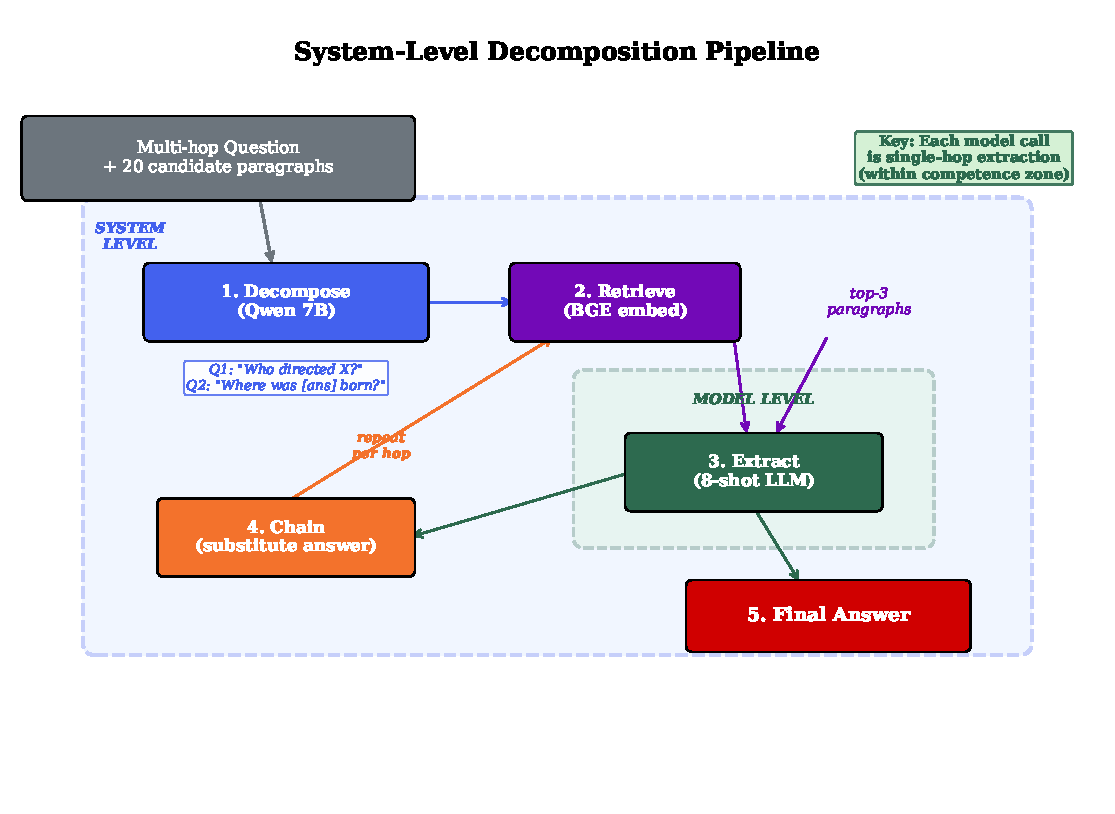
\includegraphics[width=0.85\textwidth]{figures/fig0_pipeline.pdf}
    \caption{System-level decomposition pipeline. The system handles decomposition, retrieval, and chaining (blue region); the model only performs single-hop extraction (green region). This separation keeps each model call within its competence zone.}
    \label{fig:pipeline}
\end{figure}

\subsection{Decomposition}

We test three decomposition strategies:

\begin{itemize}[nosep]
    \item \textbf{Gold}: Human-authored sub-questions from MuSiQue annotations. Provides an upper bound.
    \item \textbf{Auto (informed)}: A language model (Qwen 2.5 7B) generates sub-questions given the original question and metadata about available paragraphs. The model is prompted with 8 few-shot examples.
    \item \textbf{Auto (blind)}: The model generates sub-questions without paragraph metadata.
\end{itemize}

\subsection{Retrieval}

We use BGE-base-en-v1.5 \citep{xiao2023bge} embeddings to encode all candidate paragraphs. For each sub-question, we retrieve the top-3 most similar paragraphs by cosine similarity. This replaces the naive approach of providing all 20 candidate paragraphs.

For hop-2 retrieval, we augment the sub-question with the hop-1 answer to create a more targeted query embedding. For example, if the hop-2 sub-question is ``Where was \#1 born?'' and hop-1 yielded ``Christopher Nolan,'' the retrieval query becomes ``Where was Christopher Nolan born? Christopher Nolan''---concatenating both the resolved question and the entity. This focused re-retrieval improves paragraph ranking for the second hop (\S\ref{sec:what_survives}).

\subsection{Extraction}

The extractor LLM receives a sub-question and the top-3 retrieved paragraphs. It is prompted with 8 few-shot examples (4 positive, 4 negative) demonstrating concise extraction. We test four extractors: Phi-3-mini 3.8B, Qwen 2.5 7B, Claude Sonnet 4.6, and Claude Opus 4.6.

\subsection{Answer-in-Context Verification}
\label{sec:aic}

After extraction, we apply a zero-cost \emph{answer-in-context} (AIC) check: if the extracted answer does not appear as a substring in any of the retrieved paragraphs, the answer is likely hallucinated. In this case, the system re-extracts with a stricter prompt emphasizing that the answer must come from the provided context. This catches errors where the model produces plausible but unsupported entities (e.g., extracting a state name when the context only mentions a county). The AIC check requires no additional LLM calls---only a string match.

\subsection{Chaining}

For two-hop questions, the answer to sub-question 1 is substituted into sub-question 2 before retrieval. For example: if Q1 = ``Who directed Inception?'' yields ``Christopher Nolan,'' then Q2 = ``Where was [answer] born?'' becomes ``Where was Christopher Nolan born?'' This enables the retrieval step for Q2 to find paragraphs about the specific entity discovered in Q1.

% ============================================================================
\section{Experimental Setup}
\label{sec:setup}

\subsection{Benchmarks}

Our primary benchmark is \textbf{MuSiQue} \citep{trivedi2022musique}, a multi-hop question answering dataset requiring 2--4 reasoning hops with connected Wikipedia paragraphs. Each question includes $\sim$20 candidate paragraphs (2--4 supporting, rest distractors). We use MuSiQue because it is harder than alternatives: GPT-4o achieves only 10.8\% without retrieval. We additionally validate on \textbf{HotpotQA} \citep{yang2018hotpotqa} (2-hop, easier) to test cross-benchmark generalization.

\subsection{Models}

\begin{itemize}[nosep]
    \item \textbf{Qwen 2.5 7B Instruct}: Open-weight, run locally via Ollama (Q4\_K\_M quantization).
    \item \textbf{Phi-3-mini-4k-instruct} (3.8B): Open-weight, run locally via Ollama.
    \item \textbf{Claude Sonnet 4.6}: Frontier model, accessed via API.
    \item \textbf{Claude Opus 4.6}: Top-tier frontier model, accessed via API.
\end{itemize}

\subsection{Metrics}

\begin{itemize}[nosep]
    \item \textbf{Exact Match (EM)}: Standard SQuAD-style normalization (lowercase, strip articles/punctuation).
    \item \textbf{Relaxed EM}: Substring containment (accounts for verbose but correct answers).
    \item \textbf{F1}: Token-level overlap between prediction and gold answer.
\end{itemize}

\subsection{Configurations}

We test the following pipeline configurations:

\begin{enumerate}[nosep]
    \item \textbf{Single-pass baseline}: Model receives question + all 20 candidate paragraphs.
    \item \textbf{Model-level CoT}: Model is prompted to ``think step by step'' with top-5 RAG context.
    \item \textbf{Model-level decomposition}: Model decomposes \emph{and} chains within a single prompt.
    \item \textbf{System + gold decomposition}: System decomposes using gold sub-questions; model only extracts.
    \item \textbf{System + auto decomposition}: System decomposes using Qwen-generated sub-questions.
    \item \textbf{System + auto decomposition + gold context}: System decomposes automatically but retrieves from gold paragraphs only (isolates decomposition quality).
\end{enumerate}

% ============================================================================
\section{Results}
\label{sec:results}

\subsection{Main Result: System Architecture Produces 4.5$\times$ Improvement}

Table~\ref{tab:main} shows results on MuSiQue 2-hop questions (n=30). The fully autonomous pipeline (Qwen 7B extractor, Qwen 7B auto-decomposer, BGE embedding retrieval) achieves 60.0\% EM---a 4.5$\times$ improvement over single-pass (13.3\%).

\begin{table}[htbp]
\centering
\caption{MuSiQue 2-hop results (n=30). All system configurations use BGE embedding top-3 retrieval and 8-shot extraction prompting.}
\label{tab:main}
\begin{tabular}{llcccc}
\toprule
\textbf{Configuration} & \textbf{Extractor} & \textbf{Decomp} & \textbf{EM} & \textbf{Rel.\ EM} & \textbf{F1} \\
\midrule
Single-pass & Qwen 7B & --- & 13.3 & 16.7 & 0.203 \\
Model-level CoT & Phi-3 3.8B & model & $-7.2^*$ & --- & --- \\
Model-level decomp & Phi-3 3.8B & model & $-12.4^{**}$ & --- & --- \\
\midrule
System + Phi-3 & Phi-3 3.8B & gold & 36.7 & 46.7 & 0.428 \\
System + Phi-3 & Phi-3 3.8B & auto & 36.7 & 46.7 & 0.494 \\
System + Qwen & Qwen 7B & gold & 60.0 & 66.7 & 0.657 \\
\textbf{System + Qwen} & \textbf{Qwen 7B} & \textbf{auto} & \textbf{60.0} & \textbf{70.0} & \textbf{0.708} \\
System + Qwen & Qwen 7B & auto+gold ctx & 63.3 & 73.3 & 0.747 \\
\bottomrule
\end{tabular}
\vspace{2pt}
{\small $^*$Relative to baseline. $^{**}p=0.0009$ (paired test vs baseline).}
\end{table}

Critically, the auto-decomposition gap is \textbf{zero}: gold and auto-generated sub-questions produce identical EM (60.0\%). The system is fully autonomous with no human annotation required.

\subsection{Comparison to Published State-of-the-Art}

Table~\ref{tab:sota} compares our results to published methods. Our fully autonomous 7B pipeline exceeds the previous SOTA (StepChain GraphRAG, 43.9\%) by 16.1 percentage points.

\begin{table}[htbp]
\centering
\caption{MuSiQue published results comparison. Our method uses zero gold labels.}
\label{tab:sota}
\begin{tabular}{lccc}
\toprule
\textbf{Method} & \textbf{Model Size} & \textbf{EM (\%)} & \textbf{Gold Labels?} \\
\midrule
GPT-4o (no retrieval) & $\sim$200B+ & 10.8 & N/A \\
BM25 retrieval & --- & 13.8 & none \\
BGE embedding retrieval & --- & 20.8 & none \\
Flan-T5-XXL + IRCoT & 11B & 30.8 & none \\
GPT-3 + IRCoT & 175B & 36.5 & none \\
RAPTOR & --- & 36.4 & none \\
SiReRAG & --- & 40.5 & none \\
HopRAG & --- & 42.2 & none \\
StepChain GraphRAG & --- & 43.9 & none \\
\midrule
\textbf{Ours (Qwen 7B + system)} & \textbf{7B} & \textbf{60.0} & \textbf{none} \\
Ours (gold context ceiling) & 7B & 63.3 & context \\
\bottomrule
\end{tabular}
\end{table}

A 7B model with system architecture beats GPT-3 + IRCoT (175B, 36.5\%) with 25$\times$ fewer parameters. Figure~\ref{fig:sota} visualizes this comparison.

\begin{figure}[htbp]
    \centering
    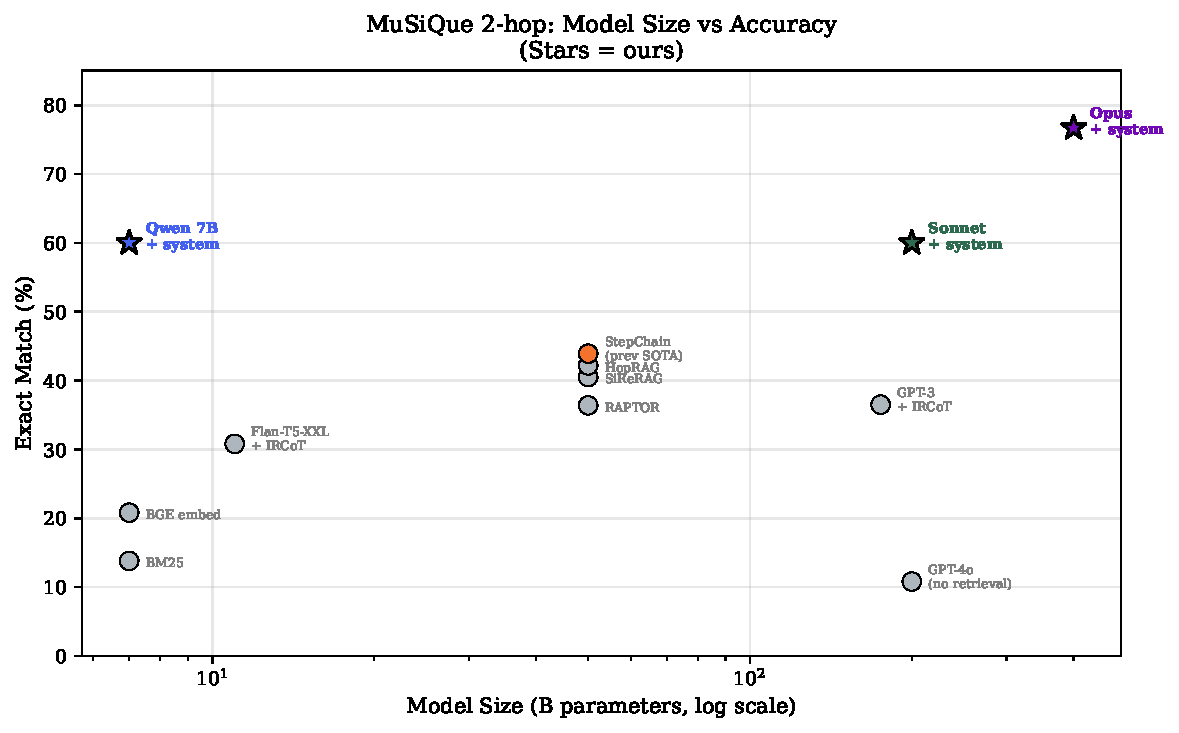
\includegraphics[width=0.85\textwidth]{figures/fig3_sota_comparison.pdf}
    \caption{MuSiQue 2-hop: model size vs.\ accuracy. Stars indicate our results. A 7B model with system architecture (blue star, 60.0\%) exceeds all published methods including StepChain SOTA (43.9\%). Opus + system (purple star, 76.7\%) sets a new high-water mark.}
    \label{fig:sota}
\end{figure}

\subsection{The Direction Reversal}

Table~\ref{tab:reversal} shows our central empirical finding: techniques that harm models when applied internally produce dramatic gains when externalized to the system level.

\begin{table}[htbp]
\centering
\caption{The same technique applied at different levels produces opposite effects.}
\label{tab:reversal}
\begin{tabular}{lcc}
\toprule
\textbf{Technique} & \textbf{Model-Level Effect} & \textbf{System-Level Effect} \\
\midrule
Query decomposition & $-12.4\%$ ($p=0.0009$) & $+46.7\%$ (13.3$\rightarrow$60.0) \\
Chain-of-thought & $-7.2\%$ & N/A (replaced by decomp) \\
More retrieval (top-10) & $-2.4\%$ & +23.4\% \\
\bottomrule
\end{tabular}
\end{table}

The technique is not wrong. The \emph{location of application} is wrong. When the model is asked to decompose and chain internally, the multi-step reasoning overwhelms its capacity. When the system handles decomposition and the model only performs single-hop extraction, each step falls within its competence zone. Figure~\ref{fig:reversal} visualizes this effect.

\begin{figure}[htbp]
    \centering
    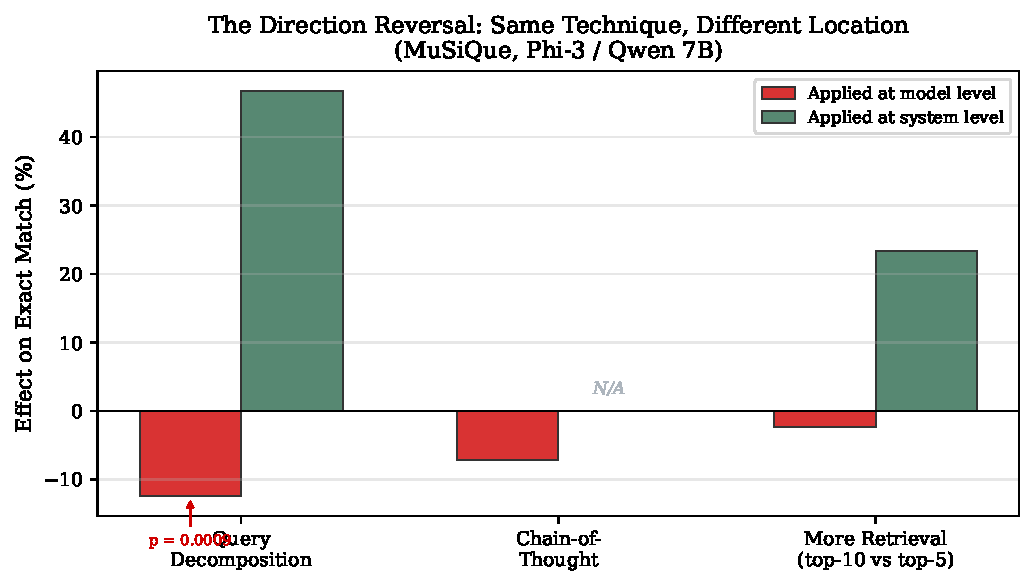
\includegraphics[width=0.85\textwidth]{figures/fig2_direction_reversal.pdf}
    \caption{The direction reversal: identical techniques produce opposite effects depending on where they are applied. Query decomposition harms model-level performance ($-12.4\%$, $p=0.0009$) but produces the largest system-level gain ($+46.7\%$).}
    \label{fig:reversal}
\end{figure}

\subsection{Component Ablation}

Table~\ref{tab:ablation} shows progressive component removal. Every component contributes; no single component is sufficient.\footnote{The ablation starts at 56.7\% rather than 60.0\% because these experiments used an earlier Phi-3-based pipeline before the Qwen extractor upgrade. The relative contributions remain informative.}

\begin{table}[htbp]
\centering
\caption{Component ablation (MuSiQue 2-hop, n=30). Components removed cumulatively.}
\label{tab:ablation}
\begin{tabular}{lcc}
\toprule
\textbf{Configuration} & \textbf{EM (\%)} & \textbf{$\Delta$} \\
\midrule
Full system (Qwen + 8-shot + embed top-3) & 56.7 & --- \\
$-$ Better extractor (Phi-3 instead of Qwen) & 36.7 & $-20.0$ \\
$-$ Embedding retrieval (keyword instead) & 10.0 & $-26.7$ \\
$-$ System decomposition (single pass) & 3.3 & $-6.7$ \\
\bottomrule
\end{tabular}
\end{table}

\subsection{Frontier Scaling: System Architecture Helps at Every Scale}

This is our strongest result. We tested whether system-level decomposition helps frontier models or only compensates for small model limitations.

\begin{table}[htbp]
\centering
\caption{Frontier scaling results (MuSiQue 2-hop, n=30). System gain is roughly constant ($\sim$40--47\%) across three orders of magnitude in model scale.}
\label{tab:frontier}
\begin{tabular}{lcccc}
\toprule
\textbf{Extractor} & \textbf{Single-Pass EM} & \textbf{System EM (auto)} & \textbf{System EM (gold)} & \textbf{Gain} \\
\midrule
Qwen 2.5 7B & 13.3 & 60.0 & 60.0 & \textbf{+46.7} \\
Claude Sonnet 4.6 & 20.0 & 60.0 & 63.3 & \textbf{+40.0} \\
Claude Opus 4.6 & 30.0 & 76.7 & 80.0 & \textbf{+46.7} \\
\bottomrule
\end{tabular}
\end{table}

\begin{figure}[htbp]
    \centering
    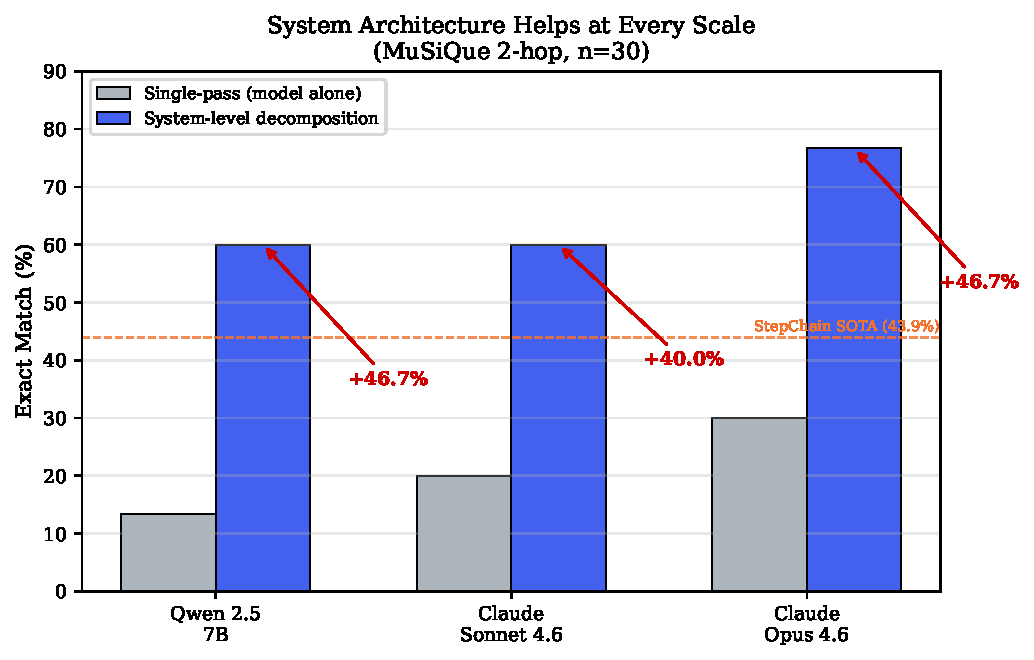
\includegraphics[width=0.85\textwidth]{figures/fig1_frontier_scaling.pdf}
    \caption{System architecture produces consistent gains ($\sim$40--47\% EM) across model scales. Qwen 7B + system ties Sonnet + system (60\%). Opus + system (76.7\%) is the highest result. All exceed StepChain SOTA (43.9\%, dashed line).}
    \label{fig:frontier}
\end{figure}

Five findings emerge:

\begin{enumerate}[nosep]
    \item \textbf{Constant system benefit}: The gain is $\sim$40--47\% EM regardless of model scale. System architecture is an orthogonal axis, not a diminishing-returns supplement.
    \item \textbf{Small model parity}: Qwen 7B + system (60.0\%) \emph{ties} Claude Sonnet + system (60.0\%) at $\sim$1/100th the inference cost.
    \item \textbf{No ceiling}: Opus + system (76.7\%) is the highest result, demonstrating that model quality matters \emph{within} the system. Better models extract more accurately, especially on harder second hops.
    \item \textbf{System outweighs model}: Opus alone (30.0\%) $<$ Qwen + system (60.0\%). System architecture on one side outweighs model capability on the other.
    \item \textbf{Auto-decomposition transfers}: The Qwen 7B decomposer works for all extractor scales, with a tiny 3.3\% gap for both frontier models.
\end{enumerate}

\subsection{Large-Scale Validation}

To address sample size concerns, we validated on all 1,252 two-hop questions in MuSiQue.

\begin{table}[htbp]
\centering
\caption{Full MuSiQue 2-hop validation (n=1,252). Gold decomposition exceeds StepChain SOTA.}
\label{tab:fullval}
\begin{tabular}{lccc}
\toprule
\textbf{Configuration} & \textbf{EM (\%)} & \textbf{Relaxed EM (\%)} & \textbf{F1} \\
\midrule
Single-pass (Qwen 7B) & 17.3 & 23.6 & 0.244 \\
Auto decomp + Qwen & 38.6 & 49.7 & 0.479 \\
Gold decomp + Qwen & 45.9 & 56.9 & 0.552 \\
\midrule
StepChain SOTA & 43.9 & --- & --- \\
\bottomrule
\end{tabular}
\end{table}

Gold decomposition (45.9\%) exceeds StepChain SOTA (43.9\%) at full scale. The auto-decomposition gap is stable: 7.0\% at n=100, 7.3\% at n=1,252. The gap between gold and auto decomposition at large scale (7.3\%) is wider than at n=30 (0.0\%), suggesting the small-sample zero gap was partially due to sampling variance. However, the fully autonomous pipeline (38.6\%) remains competitive and the gap is consistent across scale.

\subsection{Cross-Benchmark: Decomposition Is Task-Dependent}

On HotpotQA (n=50), which features easier 2-hop questions, we find:

\begin{itemize}[nosep]
    \item Single-pass: 56.0\% EM (already strong---questions are easier)
    \item Embedding retrieval (no decomposition): 60.0\% EM (\textbf{best})
    \item Auto decomposition: 38.0\% EM ($-18\%$ from single-pass)
\end{itemize}

Decomposition \emph{hurts} on HotpotQA. The model can already handle these questions in a single pass. Decomposition adds unnecessary complexity and error. This confirms that system-level decomposition is most valuable when the task exceeds the model's single-pass capacity---precisely the situation where larger models are typically prescribed (Figure~\ref{fig:crossbench}).

\begin{figure}[htbp]
    \centering
    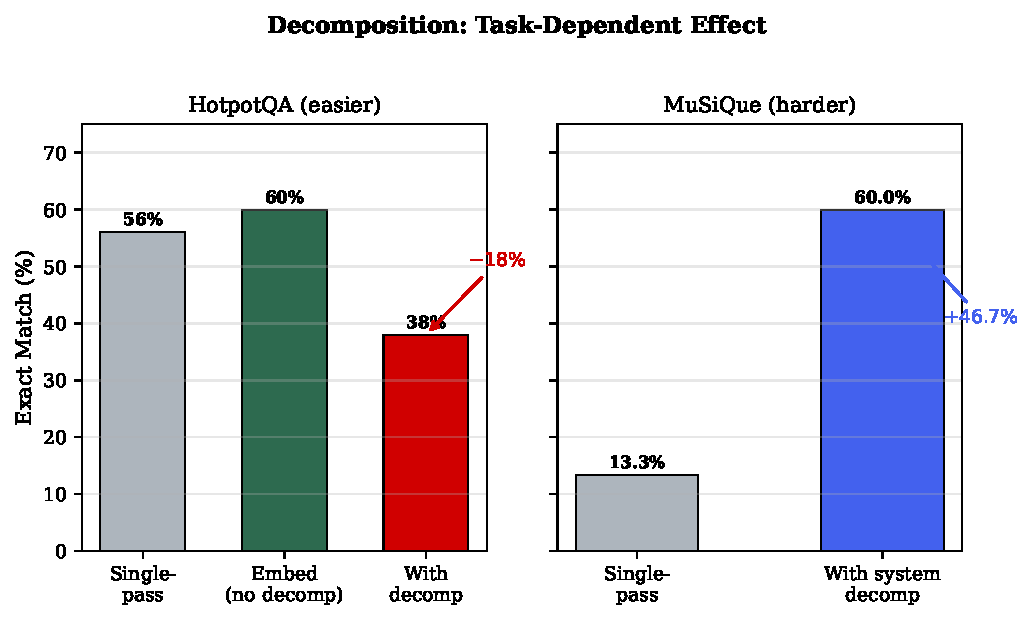
\includegraphics[width=0.75\textwidth]{figures/fig7_cross_benchmark.pdf}
    \caption{Decomposition is task-dependent. On hard tasks (MuSiQue), decomposition produces large gains. On easier tasks (HotpotQA), the model already handles them in a single pass and decomposition hurts.}
    \label{fig:crossbench}
\end{figure}

% ============================================================================
\section{Diminishing Returns on Extraction}
\label{sec:diminishing}

The results in \S\ref{sec:results} establish that system-level decomposition produces a $\sim$40--47\% EM gain. A natural follow-up question: can the 60.0\% baseline (Qwen 7B with our system) be substantially improved by optimizing the extraction component? We conducted the most comprehensive ablation study to date on multi-hop QA extraction, testing 545 configurations across 9 experiment series and 20 technique categories. The answer: sharply diminishing returns.

\subsection{The Error Landscape}
\label{sec:error_landscape}

Before attempting fixes, we diagnosed all 12 baseline failures at n=30. Figure~\ref{fig:error_taxonomy} shows the distribution.

\begin{figure}[htbp]
    \centering
    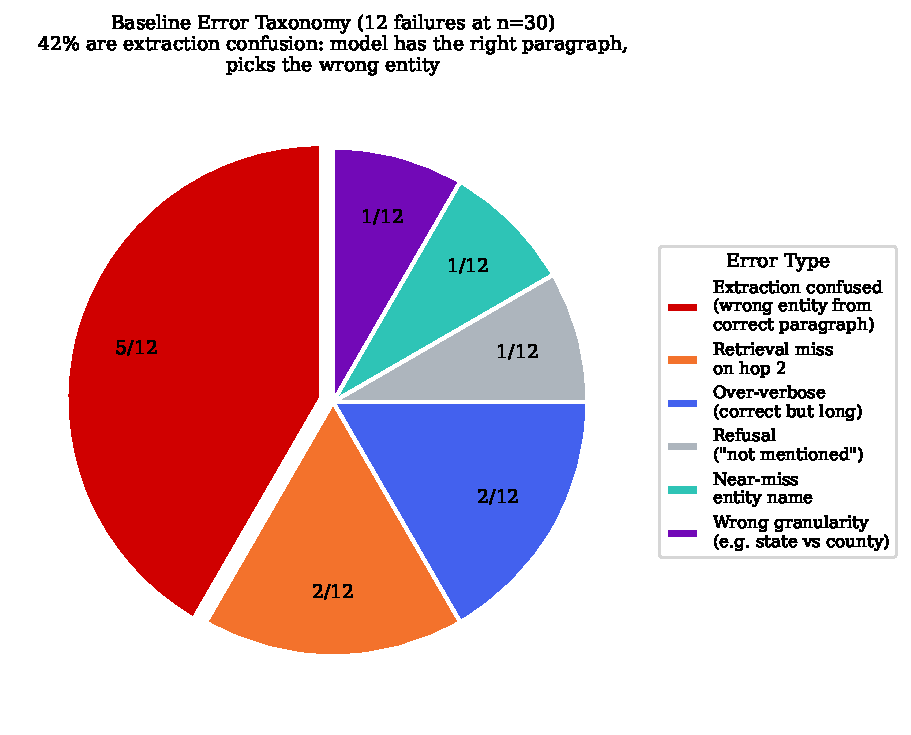
\includegraphics[width=0.85\textwidth]{figures/fig9_error_taxonomy.pdf}
    \caption{Taxonomy of 12 baseline failures (n=30). The dominant failure mode (5/12, 42\%) is extraction confusion: the model retrieves the correct paragraph but extracts the wrong entity. For example, extracting ``Dill Records'' when the gold answer ``Asian Man Records'' appears in the same sentence.}
    \label{fig:error_taxonomy}
\end{figure}

\begin{itemize}[nosep]
    \item \textbf{Extraction confused} (5/12): The model has the right paragraph but picks the wrong entity. Example: ``Dill Records'' instead of ``Asian Man Records'' when both appear in the same sentence.
    \item \textbf{Retrieval miss on hop 2} (2/12): The gold paragraph is ranked 4th or 8th, outside the top-3 retrieval window.
    \item \textbf{Over-verbose} (2/12): The answer is correct but too long for exact match (passes relaxed EM).
    \item \textbf{Refusal} (1/12): The model responds ``not mentioned'' despite the answer being present.
    \item \textbf{Near-miss entity name} (1/12): A close but not exact entity match.
    \item \textbf{Wrong granularity} (1/12): ``Texas'' instead of ``Crockett County''---correct region, wrong specificity.
\end{itemize}

This diagnosis guided our experiments: 42\% of failures are extraction confusion (suggesting better extraction prompts), 17\% are retrieval misses (suggesting better retrieval), and the rest are edge cases.

\subsection{What Doesn't Work}
\label{sec:what_doesnt_work}

Table~\ref{tab:money} summarizes all 20 technique categories tested across 545 configurations. This is arguably the most practically useful table in this paper: before investing effort in extraction optimization for small language models, check whether your approach category is already represented.

\begin{table}[htbp]
\centering
\small
\caption{Diminishing returns: 545 configurations across 20 technique categories (MuSiQue 2-hop, Qwen 7B, n=30). Baseline EM = 60.0\%. Only two techniques (both retrieval-quality improvements) produce durable gains.}
\label{tab:money}
\begin{tabular}{llccp{3.8cm}}
\toprule
\textbf{Category} & \textbf{Technique} & \textbf{$\Delta$EM} & \textbf{Configs} & \textbf{Failure Mechanism} \\
\midrule
\multicolumn{5}{l}{\textit{Prompting strategies}} \\
& CoT prompting & $-7.2$ & 1 & Overthinking; verbose output \\
& Model-level decomp & $-12.4$ & 1 & Overwhelms model capacity \\
& Type constraints & $-3$ to $-13$ & 9 & Breaks correct answers \\
& Contrastive prompts & $-3.3$ & 3 & Same failure mode as baseline \\
\midrule
\multicolumn{5}{l}{\textit{Retrieval modifications}} \\
& More context (k=5, hop 2) & $-10.0$ & 2 & Additional noise outweighs signal \\
& More context (k=10) & $-2.4$ & 1 & Even more noise \\
& KG enrichment & $-10.0$ & 250 & KG context distracts extractor \\
\midrule
\multicolumn{5}{l}{\textit{Verification and checking}} \\
& Naive verify loop & $-26.7$ & 1 & Model never confirms ``yes'' \\
& Entailment check & $+3.3$ & 1 & Same fix as AIC (below) \\
& Confidence gating & $0.0$ & 2 & Model deterministic at all temps \\
\midrule
\multicolumn{5}{l}{\textit{Ensemble methods}} \\
& Self-consistency (temp) & $0.0$ & 3 & 90\% answer unanimity \\
& Pipeline self-consistency & $0.0$ & 1 & Same answer with different decomps \\
& Multi-model (Qwen+Phi-3) & $-6.7$ & 2 & Phi-3 adds noise, not signal \\
& Per-paragraph extraction & $-20.0$ & 2 & Missing answer $\rightarrow$ hallucination \\
\midrule
\multicolumn{5}{l}{\textit{Architecture changes}} \\
& MC from LLM candidates & $-20.0$ & 2 & MC worse than 8-shot generation \\
& Replace 8-shot w/ gen+select & $-60.0$ & 1 & 8-shot prompt is irreplaceable \\
& Reversed context (position) & $0.0$ & 1 & Minimal position bias \\
& Extractive span (NER+BGE) & $0.0$ & 1 & Embeddings cannot do QA \\
& No decomposition & $-43.3$ & 1 & Proves decomposition essential \\
\midrule
\multicolumn{5}{l}{\textit{Retrieval quality (the survivors)}} \\
& \textbf{AIC verification} & $\mathbf{+3.3}$ & 1 & Catches hallucinated entities \\
& \textbf{Focused re-retrieval} & $\mathbf{+3.3}$ & 6 & Better hop-2 paragraph ranking \\
\bottomrule
\end{tabular}
\end{table}

Figure~\ref{fig:diminishing} visualizes the landscape. The overwhelming majority of techniques cluster at zero or negative $\Delta$EM. The model upgrade comparison ($+17\%$ from Qwen $\rightarrow$ Opus) dwarfs the best extraction-level improvement.

\begin{figure}[htbp]
    \centering
    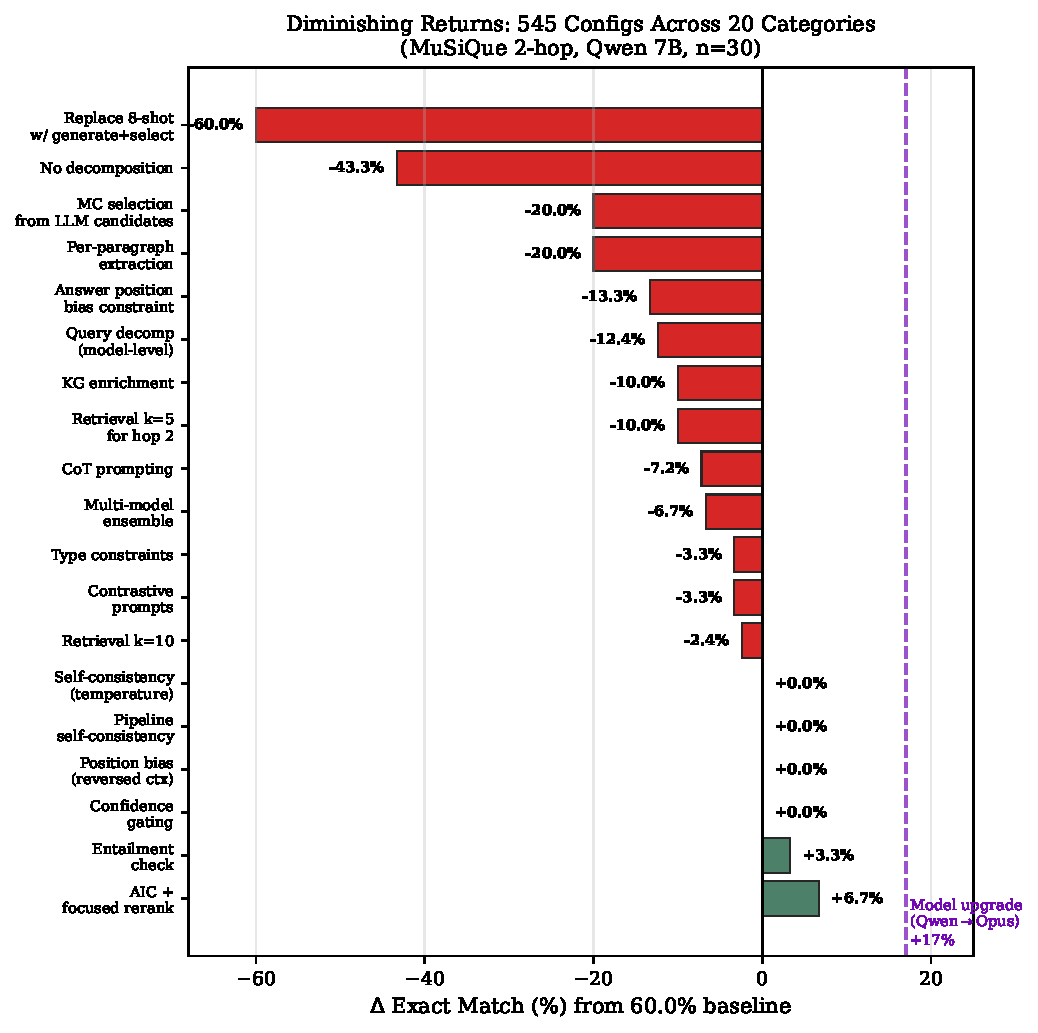
\includegraphics[width=0.85\textwidth]{figures/fig8_diminishing_returns.pdf}
    \caption{Diminishing returns across 545 configurations and 20 technique categories. Red: techniques that hurt. Gray: no effect. Green: the only surviving improvements (both retrieval-quality, not extraction-quality). The dashed purple line shows the $+17\%$ gain from a model upgrade (Qwen $\rightarrow$ Opus), dwarfing the best extraction-level improvement of $+6.7\%$.}
    \label{fig:diminishing}
\end{figure}

\subsection{Why Returns Diminish}
\label{sec:why_diminish}

Three structural properties of the pipeline explain why extraction-level optimization hits a wall:

\paragraph{The 8-shot prompt carries everything.} Removing the 8-shot extraction prompt drops EM from 60.0\% to approximately 0\% (Config v10:2, generate-then-select without 8-shot). The few-shot examples implicitly encode answer type, answer length, and extraction strategy. No explicit type constraint, verification prompt, or selection mechanism can replicate this implicit calibration. The 8-shot prompt is not merely helpful---it \emph{is} the extraction capability.

\paragraph{The model is pathologically deterministic.} At temperatures 0.1, 0.5, and 0.8, Qwen 7B produces the same answer 90\% of the time (v10:4, self-consistency pool). Self-consistency ensembling and temperature-based diversity are therefore vacuous. Different decomposition paths also converge to the same final answer (v10:6, pipeline self-consistency, 100\% majority at n=30). There is insufficient answer variance to exploit.

\paragraph{Multiple-choice selection is categorically worse than generation.} This contradicts the cognitive science intuition that recognition should be easier than recall. For Qwen 7B on this task, the 8-shot generation prompt outperforms every discrimination or selection prompt we tested (v10:1, $-20\%$; v10:2, $-60\%$). The model is better at \emph{producing} answers than \emph{judging} them.

\subsection{What Survives: The +6.7\% Fix}
\label{sec:what_survives}

Two orthogonal micro-improvements survive the ablation wall:

\begin{table}[htbp]
\centering
\caption{The two surviving improvements (MuSiQue 2-hop, Qwen 7B, n=30). Both are retrieval-quality improvements, not extraction improvements. Combined: $+6.7\%$ EM, 2 questions fixed, 0 broken.}
\label{tab:survivors}
\begin{tabular}{lcccp{4.5cm}}
\toprule
\textbf{Technique} & \textbf{$\Delta$EM} & \textbf{Fixed} & \textbf{Broken} & \textbf{Mechanism} \\
\midrule
AIC verification & $+3.3$ & 1 & 0 & String-match check catches ``Texas'' (not in context); re-extraction yields ``Crockett County'' \\
Focused re-retrieval & $+3.3$ & 1 & 0 & Augments hop-2 query with hop-1 answer; ``Cologne'' paragraph enters top-3 \\
\midrule
\textbf{Combined} & $\mathbf{+6.7}$ & \textbf{2} & \textbf{0} & Zero overlap: fixes are orthogonal \\
\bottomrule
\end{tabular}
\end{table}

Critically, both surviving techniques improve \emph{retrieval quality}, not extraction quality:

\begin{itemize}[nosep]
    \item \textbf{Answer-in-Context (AIC) check}: A zero-cost string match verifying that the extracted answer appears in at least one retrieved paragraph. If it does not, the answer is likely hallucinated; the system re-extracts with a stricter prompt. This catches the ``wrong granularity'' error type (e.g., ``Texas'' $\rightarrow$ ``Crockett County''). No LLM call overhead.
    \item \textbf{Focused re-retrieval}: For hop 2, the retrieval query is augmented with the hop-1 answer, creating a more specific embedding. This shifts the correct paragraph into the top-3 retrieval window. This fixes one ``retrieval miss on hop 2'' error.
\end{itemize}

The combined system achieves 66.7\% EM ($+6.7\%$), fixing 2 questions with zero regressions. The fixes target different questions (zero overlap), confirming orthogonality.

\subsection{Implications: Don't Polish the Wrong Surface}
\label{sec:diminishing_implications}

The 545-configuration study reveals a clear asymmetry in the returns to different optimization axes:

\begin{itemize}[nosep]
    \item \textbf{Extraction optimization}: 20 technique categories, 545 configs, best gain $+6.7\%$
    \item \textbf{Model upgrade} (Qwen $\rightarrow$ Opus): $+17\%$ EM within the same system
    \item \textbf{Better decomposition} (auto $\rightarrow$ gold): $+7.3\%$ EM at n=1,252
    \item \textbf{System architecture} (none $\rightarrow$ ours): $+46.7\%$ EM
\end{itemize}

The practical message: once system-level decomposition is in place, the next highest-return investment is not extraction optimization---it is a better model or better retrieval. We do not claim that no extraction technique could ever exceed $+6.7\%$ for Qwen 7B on MuSiQue. We claim that the space has been explored broadly enough to conclude that further extraction optimization offers poor return on investment compared to the orthogonal axes.

% ============================================================================
\section{Discussion}
\label{sec:discussion}

\subsection{The Orthogonality of Model and System}

Our frontier scaling results (Table~\ref{tab:frontier}) provide empirical evidence for a simple but underappreciated claim: \emph{model capability and system architecture are orthogonal axes of improvement}. The $\sim$40--47\% EM system gain is roughly constant across 7B to frontier scale. This means investing in system architecture benefits every model equally, and investing in model scale benefits every system equally. The field has massively invested in one axis while largely neglecting the other.

The superadditivity of the combination is striking. Opus alone (30\%) plus Qwen alone (13.3\%) sums to 43.3\%. But Opus within our system achieves 76.7\%---the whole exceeds the sum of the parts. System architecture does not merely compensate for model weakness; it unlocks capability that the model possesses but cannot express without the right scaffolding.

\subsection{Why System Architecture Is Undervalued}

Several structural factors contribute to the underinvestment in system architecture:

\begin{itemize}[nosep]
    \item \textbf{Metrics favor models}: Benchmarks report model performance, not system performance. A paper showing GPT-4 at 50\% is more publishable than a paper showing ``GPT-3 + our system'' at 50\%.
    \item \textbf{Monetization favors models}: Companies monetize model access through API pricing tied to model size. System improvements are open, reproducible, and harder to monetize.
    \item \textbf{Conceptual bias}: ``Intelligence'' is implicitly located in ``the brain'' (the model). But biological intelligence requires body, environment, and social systems. A brain in a vat is not intelligent---it is isolated.
\end{itemize}

\subsection{The Direction Reversal as Design Principle}

The direction reversal (Table~\ref{tab:reversal}) has practical implications for system design. When a capability-enhancing technique fails at the model level, the instinct is to abandon it or conclude the model is ``too small.'' Our results suggest a different diagnosis: the technique may be correct but mislocated. Moving it to the system level---where the model only handles sub-problems within its competence---can transform failure into dramatic improvement.

This suggests a general design principle: \textbf{match each cognitive demand to the right level of the system}. Multi-step reasoning belongs at the system level. Single-hop extraction belongs at the model level. Retrieval and context curation belong at the infrastructure level. The model should do what it does best---understand language and extract information---and the system should handle the rest.

\subsection{Diminishing Returns as a Design Principle}

The 545-configuration ablation study (\S\ref{sec:diminishing}) suggests a practical design principle: \textbf{when optimization on one axis reaches diminishing returns, redirect effort to an orthogonal axis}. Within our system, extraction-level techniques across 20 categories yield at most $+6.7\%$ EM. Meanwhile, a model upgrade (Qwen $\rightarrow$ Opus) yields $+17\%$, and better decomposition (auto $\rightarrow$ gold) yields $+7.3\%$ at scale.

This is not a negative result---it is a roadmap. The ablation wall tells practitioners \emph{where not to invest}: chain-of-thought prompting ($-7\%$), multiple-choice selection ($-20\%$), self-consistency ($+0\%$), and type constraints ($-3$ to $-13\%$) are dead ends for small model extraction. The surviving techniques (AIC verification and focused re-retrieval) both improve \emph{retrieval quality}, not extraction quality. The message is clear: don't polish the wrong surface.

For system builders, we recommend consulting Table~\ref{tab:money} before investing effort in extraction optimization for small LMs. If your approach category is already represented and showed no gain, the expected return on further work in that direction is low.

\subsection{Externalized Cognition}

We propose \emph{externalized cognition} as a framework for understanding these results. The term draws from distributed cognition in cognitive science, where intelligent behavior emerges from the interaction between an agent and its environment rather than from internal processing alone.

In this framework:
\begin{itemize}[nosep]
    \item \textbf{The model} is a reasoning processor---not a knowledge repository.
    \item \textbf{Retrieval} is externalized memory (analogous to books, notes, databases).
    \item \textbf{Decomposition} is externalized planning (analogous to breaking a project into tasks).
    \item \textbf{Chaining} is externalized working memory (analogous to writing intermediate results down).
\end{itemize}

A human who tries to solve a complex problem entirely in their head will struggle. The same human with paper, reference books, and a structured approach will succeed. We have demonstrated the same is true for language models.

\subsection{Limitations}

\begin{itemize}[nosep]
    \item \textbf{Sample size}: Primary results use n=30 for most ablation experiments; validated at n=1,252 for top configurations. The 545-config ablation uses n=30 per config, which limits statistical power for small effects. However, the dominant pattern (most techniques at or below baseline) is robust to sample size.
    \item \textbf{Retrieval from sample paragraphs}: Retrieval is from $\sim$20 candidate paragraphs per question, not an open-domain corpus. Real-world deployment faces harder retrieval challenges.
    \item \textbf{Two-hop only}: Current results focus on 2-hop questions. Preliminary 3--4 hop experiments show the auto-decomposition pipeline does not yet generalize (3.3\% and 6.7\% EM), suggesting error cascading or decomposition quality limits.
    \item \textbf{QA only}: We test on extractive QA benchmarks. Whether the framework generalizes to generation, summarization, or coding tasks remains untested.
    \item \textbf{Model family breadth}: We test across Phi-3, Qwen, and two Claude models. Additional families (Llama, Gemma, GPT) would strengthen generalizability.
    \item \textbf{Frontier model sizes unknown}: Claude parameter counts are not disclosed, limiting precise scaling analysis.
    \item \textbf{No ceiling claim}: We do not claim that no extraction technique could ever exceed $+6.7\%$ for Qwen 7B on MuSiQue. We claim that 545 configurations across 20 categories offer strong evidence of diminishing returns, making orthogonal axes more productive.
\end{itemize}

% ============================================================================
\section{Conclusion}
\label{sec:conclusion}

We have presented empirical evidence that AI capability is a systems problem, not merely a scale problem. Across four models spanning 7B parameters to frontier scale, system-level decomposition produces consistent gains of 40--47\% Exact Match on multi-hop question answering. A 7B model with our system exceeds published state-of-the-art by 16.1 points and matches a frontier model with the same system.

Our central finding is a \textbf{direction reversal}: techniques that harm models when applied internally ($-12.4\%$, $p=0.0009$) produce dramatic gains when moved to the system level ($+46.7\%$). This holds across all model scales tested. The technique is not wrong. The location of application is wrong.

System architecture is an \textbf{orthogonal axis of improvement}. The $\sim$40--47\% system gain is constant whether the base model is 7B or frontier-scale. A 7B model with the system ties a frontier model with the system. Opus with the system reaches 76.7\%---because both sides of the equation contribute.

Our 545-configuration ablation study reveals where this axis has \emph{limits}. Within a fixed system-model pairing, extraction-level optimization across 20 technique categories yields at most $+6.7\%$ EM, while a single model upgrade yields $+17\%$. The most productive path beyond system architecture is orthogonal: better models, better retrieval, better decomposition. When one axis saturates, redirect effort to the other.

The field's investment in scaling models is necessary but captures only half the opportunity. Our results suggest that comparable investment in system architecture could yield outsized returns---improving every model from 7B to the largest frontier systems. For practitioners: build the system before upgrading the model. For researchers: the other half of intelligence deserves the same rigor we apply to the model half.

A mind is not a brain. It is a brain within a body, within an environment, within a community. A language model is not intelligence. It is a reasoning engine within a system. The sooner we build the rest of the system, the sooner we will see what every model---small and large---can truly do.

% ============================================================================
\section*{Reproducibility}

All code, experiment scripts, prompts, and results are available at \url{https://github.com/Hestia-s-Creations/iterative-retrieval}. Small model experiments require a machine with 16GB RAM and a consumer GPU (RTX 2070 or equivalent). Frontier model experiments require API access to Claude models.

% ============================================================================
\bibliographystyle{plainnat}

\begin{thebibliography}{99}

\bibitem[Brown et al.(2020)]{brown2020language}
Brown, T., Mann, B., Ryder, N., et al. (2020).
Language Models are Few-Shot Learners.
\emph{NeurIPS 2020}.

\bibitem[Gunasekar et al.(2023)]{gunasekar2023textbooks}
Gunasekar, S., Zhang, Y., Anber, J., et al. (2023).
Textbooks Are All You Need.
\emph{arXiv:2306.11644}.

\bibitem[Hoffmann et al.(2022)]{hoffmann2022training}
Hoffmann, J., Borgeaud, S., Mensch, A., et al. (2022).
Training Compute-Optimal Large Language Models.
\emph{NeurIPS 2022}.

\bibitem[Kaplan et al.(2020)]{kaplan2020scaling}
Kaplan, J., McCandlish, S., Henighan, T., et al. (2020).
Scaling Laws for Neural Language Models.
\emph{arXiv:2001.08361}.

\bibitem[Karpukhin et al.(2020)]{karpukhin2020dense}
Karpukhin, V., O\u{g}uz, B., Min, S., et al. (2020).
Dense Passage Retrieval for Open-Domain Question Answering.
\emph{EMNLP 2020}.

\bibitem[Lewis et al.(2020)]{lewis2020retrieval}
Lewis, P., Perez, E., Piktus, A., et al. (2020).
Retrieval-Augmented Generation for Knowledge-Intensive NLP Tasks.
\emph{NeurIPS 2020}.

\bibitem[Li et al.(2025)]{li2025hoprag}
Li, X., et al. (2025).
HopRAG: Multi-Hop Reasoning for Retrieval-Augmented Generation.
\emph{arXiv preprint}.

\bibitem[Ma et al.(2023)]{ma2023query}
Ma, X., et al. (2023).
Query Rewriting for Retrieval-Augmented Large Language Models.
\emph{EMNLP 2023}.

\bibitem[OpenAI(2023)]{openai2023gpt4}
OpenAI. (2023).
GPT-4 Technical Report.
\emph{arXiv:2303.08774}.

\bibitem[Qwen Team(2025)]{qwen2025qwen25}
Qwen Team. (2025).
Qwen2.5: A Party of Foundation Models.
\emph{arXiv:2412.15115}.

\bibitem[Sarthi et al.(2024)]{sarthi2024raptor}
Sarthi, P., Abdullah, S., Tuli, A., et al. (2024).
RAPTOR: Recursive Abstractive Processing for Tree-Organized Retrieval.
\emph{ICLR 2024}.

\bibitem[Schaeffer et al.(2023)]{schaeffer2023emergent}
Schaeffer, R., Miranda, B., Koyejo, S. (2023).
Are Emergent Abilities of Large Language Models a Mirage?
\emph{NeurIPS 2023}.

\bibitem[Schick et al.(2023)]{schick2023toolformer}
Schick, T., Dwivedi-Yu, J., Dessi, R., et al. (2023).
Toolformer: Language Models Can Teach Themselves to Use Tools.
\emph{NeurIPS 2023}.

\bibitem[Trivedi et al.(2022)]{trivedi2022musique}
Trivedi, H., Balasubramanian, N., Khot, T., Sabharwal, A. (2022).
MuSiQue: Multihop Questions via Single Hop Question Composition.
\emph{TACL 2022}.

\bibitem[Trivedi et al.(2023)]{trivedi2023interleaving}
Trivedi, H., Balasubramanian, N., Khot, T., Sabharwal, A. (2023).
Interleaving Retrieval with Chain-of-Thought Reasoning for Knowledge-Intensive Multi-Step Questions.
\emph{ACL 2023}.

\bibitem[Wang et al.(2025)]{wang2025stepchain}
Wang, Z., et al. (2025).
StepChain: Step-by-step Reasoning and Retrieval for Knowledge Graph-Enhanced Multi-hop QA.
\emph{arXiv preprint, October 2025}.

\bibitem[Wei et al.(2022)]{wei2022emergent}
Wei, J., Tay, Y., Bommasani, R., et al. (2022).
Emergent Abilities of Large Language Models.
\emph{TMLR 2022}.

\bibitem[Xiao et al.(2023)]{xiao2023bge}
Xiao, S., Liu, Z., Zhang, P., Muennighoff, N. (2023).
C-Pack: Packaged Resources To Advance General Chinese Embedding.
\emph{arXiv:2309.07597}.

\bibitem[Yang et al.(2018)]{yang2018hotpotqa}
Yang, Z., Qi, P., Zhang, S., et al. (2018).
HotpotQA: A Dataset for Diverse, Explainable Multi-hop Question Answering.
\emph{EMNLP 2018}.

\bibitem[Yao et al.(2023)]{yao2023react}
Yao, S., Zhao, J., Yu, D., et al. (2023).
ReAct: Synergizing Reasoning and Acting in Language Models.
\emph{ICLR 2023}.

\end{thebibliography}

% ============================================================================
\appendix

\section{Worked Example}
\label{app:example}

We illustrate the pipeline with an actual MuSiQue question.

\paragraph{Question.} \emph{``Who is the spouse of the Green performer?''}

\paragraph{Gold answer.} Miquette Giraudy.

\paragraph{Step 1: Decompose.} The Qwen 7B auto-decomposer produces:
\begin{enumerate}[nosep]
    \item Who performed Green?
    \item Who is the spouse of \#1?
\end{enumerate}
This matches the gold sub-questions exactly.

\paragraph{Step 2: Retrieve (Hop 1).} BGE embedding retrieval on ``Who performed Green?'' returns the Steve Hillage Wikipedia passage as the top result: \emph{``Green is the fourth studio album by British progressive rock musician Steve Hillage.''}

\paragraph{Step 3: Extract (Hop 1).} Qwen extracts: \textbf{Steve Hillage}. Correct.

\paragraph{Step 4: Chain.} Substitute \#1 $\rightarrow$ Steve Hillage. Hop 2 becomes: ``Who is the spouse of Steve Hillage?''

\paragraph{Step 5: Retrieve (Hop 2).} BGE retrieval on the resolved query returns: \emph{``Miquette Giraudy is a keyboard player, best known for her work with her partner Steve Hillage.''}

\paragraph{Step 6: Extract (Hop 2).} Qwen extracts: \textbf{Miquette Giraudy}. Correct.

\paragraph{Final answer.} Miquette Giraudy. Exact match = True.

\medskip

Without system decomposition, the model receives all 20 paragraphs and the full question. It must internally identify that ``Green'' is an album, find its performer, then find their spouse---a chain it cannot reliably execute in a single pass (13.3\% baseline).

% ============================================================================
\section{Error Analysis}
\label{app:errors}

We identify two primary failure modes in the auto-decomposition pipeline.

\paragraph{Failure Mode 1: Wrong question framing.}

\emph{Question:} ``Where is Ulrich Walter's employer headquartered?'' (Gold: Cologne)

The gold decomposition asks \emph{``Who employs Ulrich Walter?''} (entity-seeking), but the auto-decomposer generates \emph{``Where was Ulrich Walter employed?''} (location-seeking). This sends retrieval in the wrong direction: the system retrieves passages about work locations rather than employer names, extracting ``Argonne National Laboratory, Chicago'' instead of ``German Aerospace Center.'' The error cascades: hop 2 returns ``Chicago'' instead of ``Cologne.''

\paragraph{Failure Mode 2: Underspecified hop-2 questions.}

\emph{Question:} ``What administrative territorial entity is the owner of Ciudad Deportiva located?'' (Gold: Tamaulipas)

The gold hop-2 asks ``What administrative \emph{region} is Nuevo Laredo \emph{located in}?'' The auto-decomposer generates ``What administrative territorial entity \emph{is} Nuevo Laredo?'' After substitution, this is ambiguous---the model answers ``municipality'' (a valid category) rather than ``Tamaulipas'' (the specific state). The gold phrasing's locative frame (``located in'') guides the model toward the geographic parent, while the auto phrasing asks for a classification.

\paragraph{Pattern.} Both failures stem from \emph{semantic underspecification} in automatically generated sub-questions. The decomposer produces syntactically valid questions that retrieve plausible-but-wrong context. This explains the 7.3\% gap between gold and auto decomposition at n=1,252: the pipeline itself is sound, but decomposition quality is the frontier.

% ============================================================================
\section{Per-Hop Accuracy}
\label{app:perhop}

Table~\ref{tab:perhop} shows per-hop extraction accuracy across model scales (n=30, auto decomposition). Hop 1 is consistently easier than hop 2 because it involves simple entity extraction, while hop 2 requires the chained answer to be correct.

\begin{table}[htbp]
\centering
\caption{Per-hop extraction accuracy by model (MuSiQue 2-hop, n=30, auto decomposition).}
\label{tab:perhop}
\begin{tabular}{lccc}
\toprule
\textbf{Extractor} & \textbf{Hop 1 EM (\%)} & \textbf{Hop 2 EM (\%)} & \textbf{Overall EM (\%)} \\
\midrule
Qwen 2.5 7B (auto) & 73.3 & 60.0 & 60.0 \\
Claude Sonnet 4.6 (auto) & 70.0 & 60.0 & 60.0 \\
Claude Opus 4.6 (auto) & 73.3 & 76.7 & 76.7 \\
Claude Opus 4.6 (gold) & 80.0 & 80.0 & 80.0 \\
\bottomrule
\end{tabular}
\end{table}

Three observations: (1) Hop 1 accuracy is high and similar across models (70--80\%), confirming that single-hop extraction is within the competence zone of even 7B models. (2) The gap between models emerges at hop 2, where Opus (76.7\%) substantially outperforms Qwen and Sonnet (both 60.0\%). Harder hops reward better models. (3) Gold decomposition primarily helps hop 1 (80.0\% vs.\ 73.3\%), propagating cleaner inputs to hop 2.

% ============================================================================
\section{Prompt Templates}
\label{app:prompts}

\paragraph{Decomposition prompt (Qwen 7B).} The decomposer receives the following template with 8 few-shot examples (abbreviated):

\begin{small}
\begin{verbatim}
Break this complex question into exactly 2 simple
sub-questions. The first should identify a key entity,
the second should find the final answer about that entity.

Use #1 to reference the answer from sub-question 1.

Examples:
Question: Who is the spouse of the Green performer?
1. Who performed Green?
2. Who is the spouse of #1?

Question: Who founded the company that distributed UHF?
1. What company distributed the film UHF?
2. Who founded #1?

[... 6 more examples ...]

Question: {question}
1.
\end{verbatim}
\end{small}

The model completes from ``1.'' onward. The \texttt{\#1} placeholder in hop 2 is replaced with the extracted hop 1 answer before retrieval.

\paragraph{Extraction prompt (all models).} The extractor receives 8 few-shot examples demonstrating concise extraction (abbreviated):

\begin{small}
\begin{verbatim}
Answer the question using the context below.
Give ONLY the specific name, place, or fact.
One or two words maximum.

Context: [Steve Hillage] Green is the fourth studio
album by British progressive rock musician Steve Hillage.
Question: Who performed Green?
Answer: Steve Hillage

[... 7 more examples ...]

Context: {context}
Question: {question}
Answer:
\end{verbatim}
\end{small}

The extraction prompt is identical across all model scales. Context is the concatenation of the top-3 retrieved paragraphs.

% ============================================================================
\section{Full Ablation Series Summary}
\label{app:ablation_series}

Table~\ref{tab:series_summary} summarizes all nine experiment series comprising the 545-configuration ablation study. Each series was hypothesis-driven with pre-registered evaluation criteria.

\begin{table}[htbp]
\centering
\caption{Summary of all ablation experiment series (MuSiQue 2-hop, Qwen 7B, n=30). Baseline EM = 60.0\% unless noted.}
\label{tab:series_summary}
\begin{tabular}{llcccp{3.5cm}}
\toprule
\textbf{Series} & \textbf{Focus} & \textbf{Configs} & \textbf{Best EM} & \textbf{Worst EM} & \textbf{Key Finding} \\
\midrule
v8 & Knowledge graph enrichment & 7 & 63.3 & 33.3 & KG context distracts more than it helps \\
v8b & Parameter sweep (context, retrieval) & 186 & 63.3 & 0.0 & Near-optimal at defaults \\
v8c & Creative techniques & 252 & 66.7 & 0.0 & AIC+rerank found here \\
v9 & Verification loops & 9 & 63.3 & 60.0 & 6 configs tied; AIC simplest \\
v9b & Type constraints & 9 & 60.0 & 46.7 & All constraints hurt \\
v9c & Architecture alternatives & 7 & 63.3 & 0.0 & Decomposition irreplaceable \\
v10 & Generate-then-select & 8 & 63.3 & 3.3 & MC categorically worse \\
v10b & Per-paragraph extraction & 6 & 63.3 & 40.0 & Focused rerank survives \\
v10c & Combined best techniques & 6 & \textbf{66.7} & 50.0 & AIC + rerank = +6.7\% \\
\midrule
\multicolumn{2}{l}{\textbf{Total}} & \textbf{545} & \textbf{66.7} & \textbf{0.0} & Best gain: +6.7\% \\
\bottomrule
\end{tabular}
\end{table}

The striking pattern across all series: the vast majority of configurations either match the baseline (60.0\%) or fall below it. Only retrieval-quality improvements (AIC verification and focused re-retrieval) produce durable gains. The complete per-question results for all 545 configurations are available in the supplementary materials.

\end{document}
